% !TEX TS-program = xelatex
% !TEX program = xelatex
% !TEX encoding = UTF-8 Unicode

\documentclass[12pt]{article}

\usepackage{fontspec}
\usepackage{ifxetex}
\usepackage[margin=1in]{geometry}
\usepackage{enumitem}
\usepackage{setspace}
\usepackage{fancyhdr}
\usepackage{graphicx}
\usepackage{hyperref}
\usepackage{longtable}
\usepackage{booktabs}
\usepackage{caption}
\usepackage{array}

\setstretch{1.15}

% Thai font settings (XeLaTeX)
\IfFontExistsTF{Laksaman}{
  \setsansfont{Laksaman}[
    BoldFont       = Laksaman Bold,
    ItalicFont     = Laksaman Italic,
    BoldItalicFont = Laksaman Bold Italic
  ]
  \setmainfont{Laksaman}[
    BoldFont       = Laksaman Bold,
    ItalicFont     = Laksaman Italic,
    BoldItalicFont = Laksaman Bold Italic
  ]
}{
  \setsansfont[
    Path           = ./fonts/,
    UprightFont    = Laksaman.ttf,
    BoldFont       = Laksaman-Bold.ttf,
    ItalicFont     = Laksaman-Italic.ttf,
    BoldItalicFont = Laksaman-BoldItalic.ttf
  ]{Laksaman.ttf}
  \setmainfont[
    Path           = ./fonts/,
    UprightFont    = Laksaman.ttf,
    BoldFont       = Laksaman-Bold.ttf,
    ItalicFont     = Laksaman-Italic.ttf,
    BoldItalicFont = Laksaman-BoldItalic.ttf
  ]{Laksaman.ttf}
}

% Thai line breaking (XeLaTeX only)
\ifxetex
  \XeTeXlinebreaklocale "th"
  \XeTeXlinebreakskip = 0pt plus 1pt
\fi

% ========== HEADER & FOOTER ============
\pagestyle{fancy}
\fancyhf{}
\fancyfoot[R]{\thepage}
\renewcommand{\headrulewidth}{0pt}

% ================= DOCUMENT BEGINS =================
\begin{document}

% ================= TITLE PAGE =================
\begin{center}
    {\Large\bfseries รายงานฉบับสมบูรณ์โครงงานรวบยอดวิศวกรรมคอมพิวเตอร์ 2}\\[0.5pc]
    {\Large\bfseries CEDT Capstone Project Final Report}\\[2pc]
    
    {\large\bfseries เรื่อง}\\[0.5pc]
    {\large โครงการไอคิว: แพลตฟอร์มการจัดการความรู้ด้วยการสืบค้นแบบอิงบริบท} \\[0.3pc]
    {\large Project AiQ: Intelligence That Drives Execution} \\[2pc]
    
    {\large\bfseries โดย}\\[0.5pc]
    \begin{tabular}{ll}
        นายชวินทร์ เลิศสวาย & 6633047821 \\
        นายธนิตย์ ยอดสิรวงษ์ & 6633104921 \\
        นายณัฐพล ธีรยุทธวงศ์ & 6633072421 \\
        นายพีระภัทร์ พัชรมณี & 6633176021 \\
        นายปุราณ ประเสริฐไทย & 6633154221 \\
    \end{tabular}\\[2pc]
    
    {\large\bfseries อาจารย์ที่ปรึกษา}\\[0.5pc]
    ผศ. ดร. สุกรี สินธุภิญโญ \\
    รศ. ดร. ทวิทิวา เซนีวงศ์ ณ อยุธยา \\
    คุณชะนินทร อัศววิชัยโรจน์ (SCB TechX) \\
    คุณเจษฎา วีรเดชกัมพล (SCB TechX) \\[2pc]
    
    รายงานนี้เป็นส่วนหนึ่งของวิชา 2110489 โครงงานรวบยอดวิศวกรรมคอมพิวเตอร์ 2\\
    ภาควิชาวิศวกรรมคอมพิวเตอร์ คณะวิศวกรรมศาสตร์ จุฬาลงกรณ์มหาวิทยาลัย\\
    ประจำปีการศึกษา 2568
\end{center}

\newpage

% =============== ABSTRACT (THAI) ===========
\section*{บทคัดย่อ}
\addcontentsline{toc}{section}{บทคัดย่อ}
โครงงานนี้มีชื่อว่า \textit{โครงการไอคิว (Project AiQ)} หรือ "Intelligence That Drives Execution" มุ่งเน้นการแก้ปัญหาที่สำคัญเรื่องความรู้ภายในองค์กรที่กระจัดกระจาย (Fragmented Enterprise Knowledge) ซึ่งถูกเก็บไว้ในระบบต่างๆ เช่น SharePoint โดยการออกแบบ Knowledge Hub ที่ขับเคลื่อนด้วย AI ซึ่งมีความปลอดภัยและขยายตัวได้ เพื่อส่งเสริมการสืบค้นข้อมูลอัตโนมัติและเพิ่มประสิทธิภาพในองค์กร

เพื่อให้บรรลุเป้าหมายนี้ แนวทางที่นำเสนอประกอบด้วยการออกแบบและพัฒนาระบบ Retrieval-Augmented Generation (RAG) โดยมุ่งเน้นไปที่กระบวนการจัดการข้อมูล (Data Ingestion) และการเตรียมข้อมูล (Preparation Pipeline) ที่มีความสามารถในการขยายตัว ซึ่งใช้เทคนิค GraphRAG ในการจัดโครงสร้างเนื้อหาจากแหล่งข้อมูลในองค์กรอย่างปลอดภัย

ผลการดำเนินงานประกอบด้วยการออกแบบทางเทคนิคอย่างละเอียด การพัฒนากระบวนการจัดการข้อมูลที่มีระบบความปลอดภัยพื้นฐานแบบ Single Sign-On (SSO) ระบบ RAG Web Chat รุ่นต้นแบบ (MVP) และการพิสูจน์ทางวิชาการถึงสถาปัตยกรรม RAG รวมถึงประโยชน์ในเชิงอุตสาหกรรมผ่านการเพิ่มประสิทธิภาพและการรวบรวมความรู้ให้เป็นระบบเดียว โดยระบบสามารถทำค่า Mean Reciprocal Rank (MRR) ได้ที่ 0.82 และ Recall@5 ที่ 0.88

\textbf{คำสำคัญ:} RAG, การจัดการความรู้, การจัดการข้อมูล, AI ในองค์กร, GraphRAG

\newpage

% =============== ABSTRACT (ENGLISH) ===========
\section*{Abstract}
\addcontentsline{toc}{section}{Abstract}
This project, Project AiQ - "Intelligence That Drives Execution", addresses the critical problem of fragmented enterprise knowledge scattered across systems like SharePoint, by designing a secure and scalable AI-driven Knowledge Hub to automate retrieval and improve organizational efficiency.

To achieve this, the proposed solution involves designing and implementing a Retrieval-Augmented Generation (RAG) system, specifically focusing on a scalable data ingestion and preparation pipeline that utilizes GraphRAG techniques to securely structure content from enterprise sources.

The expected outcomes include a detailed technical design, an implemented data pipeline with foundational Single Sign-On (SSO) security, a minimal RAG Web Chat MVP, and significant contributions to both academic validation of the RAG architecture and industrial benefits through improved efficiency and knowledge consolidation. Final evaluation showed a Mean Reciprocal Rank (MRR) of 0.82 and a Recall@5 of 0.88, with an average end-to-end latency of 5.4 seconds.

\textbf{Keywords:} RAG, Knowledge Management, Data Ingestion, Enterprise AI, GraphRAG

\newpage

% =============== TABLE OF CONTENTS ===========
\tableofcontents
\newpage

% =============== SECTION 1 ===========
\section{Introduction \& Problem Definition}

\subsection{Background \& Motivation}
Modern enterprise environments, including organizations that manage large and complex projects like \textbf{SCB TechX}, often face a common problem: important project information is \textbf{scattered across many different systems}. Emails, shared file drives, and internal tools such as SharePoint all contain pieces of knowledge, but none of them provide a complete picture. As a result, finding the right information becomes slow, inconvenient, and sometimes confusing.

To solve this, organizations are moving toward a \textbf{Knowledge Hub} concept, which requires a system that not only consolidates data but also provides intelligent access. The central challenge, which motivates this research-focused project, is the initial step: how to securely and efficiently ingest this fragmented data and transform it into a unified, queryable knowledge base. By creating a robust ingestion and preparation pipeline early on, we aim to lay the groundwork for using AI to automate knowledge retrieval, thereby addressing inefficiency issues and ensuring project continuity.

\subsection{Problem Statement}
The core engineering problem is to design, research, and validate the technical foundation for a secure and scalable AI-driven knowledge management platform. Specifically, the problem centers on:
\begin{enumerate}
    \item Designing a robust content extraction and preparation pipeline that can handle data from enterprise-level sources (e.g., SharePoint) and structure it for semantic search.
    \item Formulating a security strategy that integrates with existing enterprise authentication methods, such as SSO (Single Sign-On).
    \item Integrating the AI and Distributed Systems disciplines to ensure the initial data ingestion architecture is scalable and reliable, which is a complex requirement for real-world enterprise deployment.
\end{enumerate}

\subsection{Objectives}
The project aims to achieve the following clear, measurable goals in a phased, two-semester approach:
\begin{enumerate}
    \item \textbf{Research and Design (Capstone I Focus):} Conduct comprehensive research on current RAG architectures, perform a gap analysis of existing knowledge management systems, and deliver a detailed technical design for the entire system, emphasizing the data ingestion and content extraction pipeline.
    \item \textbf{Data Preparation Pipeline Development (Implementation Focus):} Design and implement a scalable data ingestion and preparation pipeline capable of securely connecting to and extracting content from a primary enterprise source (e.g., SharePoint).
    \item \textbf{Foundational Integration (Implementation Focus):} Implement the foundational security integration to support Single Sign-On (SSO), ensuring secure user access to the system.
    \item \textbf{Evaluation:} Define key performance metrics for the data pipeline (e.g., latency, throughput) and the RAG model's accuracy, with testing to commence in Capstone II.
\end{enumerate}

\subsection{Scope \& Limitations}
\textbf{Scope:}
\begin{enumerate}
    \item Research \& Proposal (Capstone I): Deliver a full written proposal and research review.
    \item Data Ingestion \& Preparation: Design and implement the ingestion of unstructured and semi-structured data from SharePoint and a general file upload feature. This includes content extraction, chunking, and embedding.
    \item Security Foundation: Implement Single Sign-On (SSO) for secure user authentication.
    \item Interface: Develop a minimal Web Chat MVP with basic prompt and response functionality to demonstrate RAG output.
\end{enumerate}

\textbf{Limitations:}
\begin{enumerate}
    \item Initial data ingestion implementation will focus on one primary enterprise source (SharePoint/Xhive).
    \item Advanced access control mechanisms (e.g., RBAC) are considered complex and will be scaled back to basic authentication checks (SSO) as advanced access control is considered a future enhancement.
    \item Advanced user-facing features (e.g., multi-channel integration via LINE/MS Teams) are out-of-scope for the MVP and reserved for future work.
\end{enumerate}

\subsection{Expected Benefits}
\textbf{Academic/Technical Benefit:}
\begin{enumerate}
    \item \textbf{Validated Architecture:} Deliver a thoroughly researched and documented architecture for a complex enterprise RAG system.
    \item \textbf{Data Pipeline Expertise:} Provide practical experience in designing and implementing a robust data ingestion pipeline that handles real-world, messy, and large-scale organizational data.
    \item \textbf{RAG Optimization:} Provide a testbed for evaluating the performance implications of different RAG components (e.g., chunking strategies, re-ranking).
\end{enumerate}

\textbf{Industrial/Professional Benefit:}
\begin{enumerate}
    \item \textbf{Efficiency:} Lay the foundation to reduce the time spent searching for information, leading to eventual cost savings and improved team agility.
    \item \textbf{Knowledge Consolidation:} Create a centralized platform that turns scattered documentation into an accessible Knowledge Hub.
    \item \textbf{Streamlined Onboarding:} Improve the onboarding process for new joiners by providing an immediate, centralized, and intelligent way to access project history and essential internal knowledge.
\end{enumerate}

\subsection{Stakeholders}
Primary stakeholders include:
\begin{itemize}
    \item \textbf{Employees of SCB TechX:} End-users who require efficient access to project history and internal knowledge.
    \item \textbf{Project Managers:} Who benefit from consolidated data for better decision-making and project continuity.
    \item \textbf{System Architects:} Interested in the scalability and reliability of the modular AI infrastructure.
    \item \textbf{New Joiners:} Who benefit from a streamlined onboarding process via the Knowledge Hub.
\end{itemize}

% =============== SECTION 2 ===========
\section{Related Theory and Research}

\subsection{Review of Existing Knowledge}
In large-scale enterprise environments, knowledge is generally locked within different repositories, such as emails, cloud drives, or collaboration platforms, which makes the extraction of information less efficient. The traditional approach to Knowledge Management is based on keyword indexing, such as Inverted Indices, which fail to capture the semantic intent of user queries or contextual relationships between documents \cite{furnas1987vocabulary}.

To overcome these limitations, Retrieval-Augmented Generation (RAG) has emerged as a standard architecture. RAG enhances Large Language Models (LLMs) by retrieving relevant data from a private knowledge base (the Vector Store) before generating an answer \cite{lewis2021retrieval}. Current research emphasizes the need for high-fidelity ingestion pipelines that combine Vector Embeddings with Graph/Relational Structures (GraphRAG) to maximize context preservation \cite{edge2024local}.

\subsection{Comparison with Existing Systems}
\begin{itemize}
    \item \textbf{Level 1: Legacy Keyword Search:} Matches exact keywords; returns file lists rather than answers.
    \item \textbf{Level 2: Naive/Generic RAG Implementations:} Uses fixed-window chunking; suffers from context fragmentation and hallucinations \cite{gao2023retrieval}.
    \item \textbf{Level 3: The Proposed Pipeline-Centric System:} Prioritizes the Data Ingestion Layer using advanced parsers (Docling \cite{docling2024}) to preserve document hierarchy and structural integrity.
\end{itemize}

\subsection{Gap Analysis}
\begin{itemize}
    \item \textbf{The Ingestion Gap:} Lack of robust pipelines designed to handle "messy" enterprise data formats while preserving semantic structure.
    \item \textbf{The Synchronization Gap:} Critical shortage of systems capable of Real-time Synchronization (e.g., via SharePoint Webhooks and RabbitMQ).
    \item \textbf{The Contextual Gap:} Standard vector search flattens data, losing relational context. Requires GraphRAG-style extraction to preserve relationships.
\end{itemize}

\subsection{Linkage to Project}
Project AiQ addresses these gaps by:
\begin{enumerate}
    \item \textbf{Optimized Data Ingestion:} Transforming unstructured data from Xhive/SharePoint into high-quality assets.
    \item \textbf{Automated Knowledge Synchronization:} Monitoring source repositories for near real-time updates.
    \item \textbf{Hybrid Data Representation:} Combining vector search with structural metadata understanding.
\end{enumerate}

% =============== SECTION 3 ===========
\section{System Design}

\subsection{System Overview}
The proposed system is an AI-powered Chatbot Application for searching and answering questions from a Document Database. Users inquire with Natural Language through a Chat Interface. The system processes the request using RAG combined with GraphRAG principles to retrieve relevant content based on both semantic similarity and structural data relationships.

\subsection{Components}
\begin{itemize}
    \item \textbf{Frontend Application (Next.js/React):} Handles User Interaction and Citations.
    \item \textbf{Backend Orchestrator (NestJS):} API Gateway, Session Management, and Routing.
    \item \textbf{AI Engine (CrewAI/FastAPI):} Multi-agent cognitive processing for selective reading and reasoning.
    \item \textbf{Embedding Service (FastAPI):} Manages vector operations (BGE-M3) and Qdrant database access.
    \item \textbf{Data Ingestion Service (FastAPI/RabbitMQ):} Performs ETL, Modality Detection, and advanced Chunking (Docling).
    \item \textbf{File Storage Service (FastAPI/MinIO):} Intermediary for Object Storage management.
    \item \textbf{SharePoint Webhook Service (FastAPI):} Listener for external integration events.
\end{itemize}

\subsection{Constraints Considered}
\begin{enumerate}
    \item \textbf{Latency in Agentic Workflow:} Addressed via Progress Streaming and asynchronous background tasks.
    \item \textbf{Context Granularity:} Solved using the GraphRAG technique and Custom Agent Tools (Sliding Window Reader).
    \item \textbf{Data Consistency:} Guaranteed by linked CRUD operations through RabbitMQ and Webhooks.
    \item \textbf{LLM Safety \& Guardrails:} Implemented via Input/Output validation layers.
    \item \textbf{Complex Document Structure:} Handled by the Modality Detection process and Multilingual-compatible embeddings.
    \item \textbf{External Dependencies:} Mitigated by modular design and internal data buffering.
\end{enumerate}

\begin{figure}[ht]
    \centering
    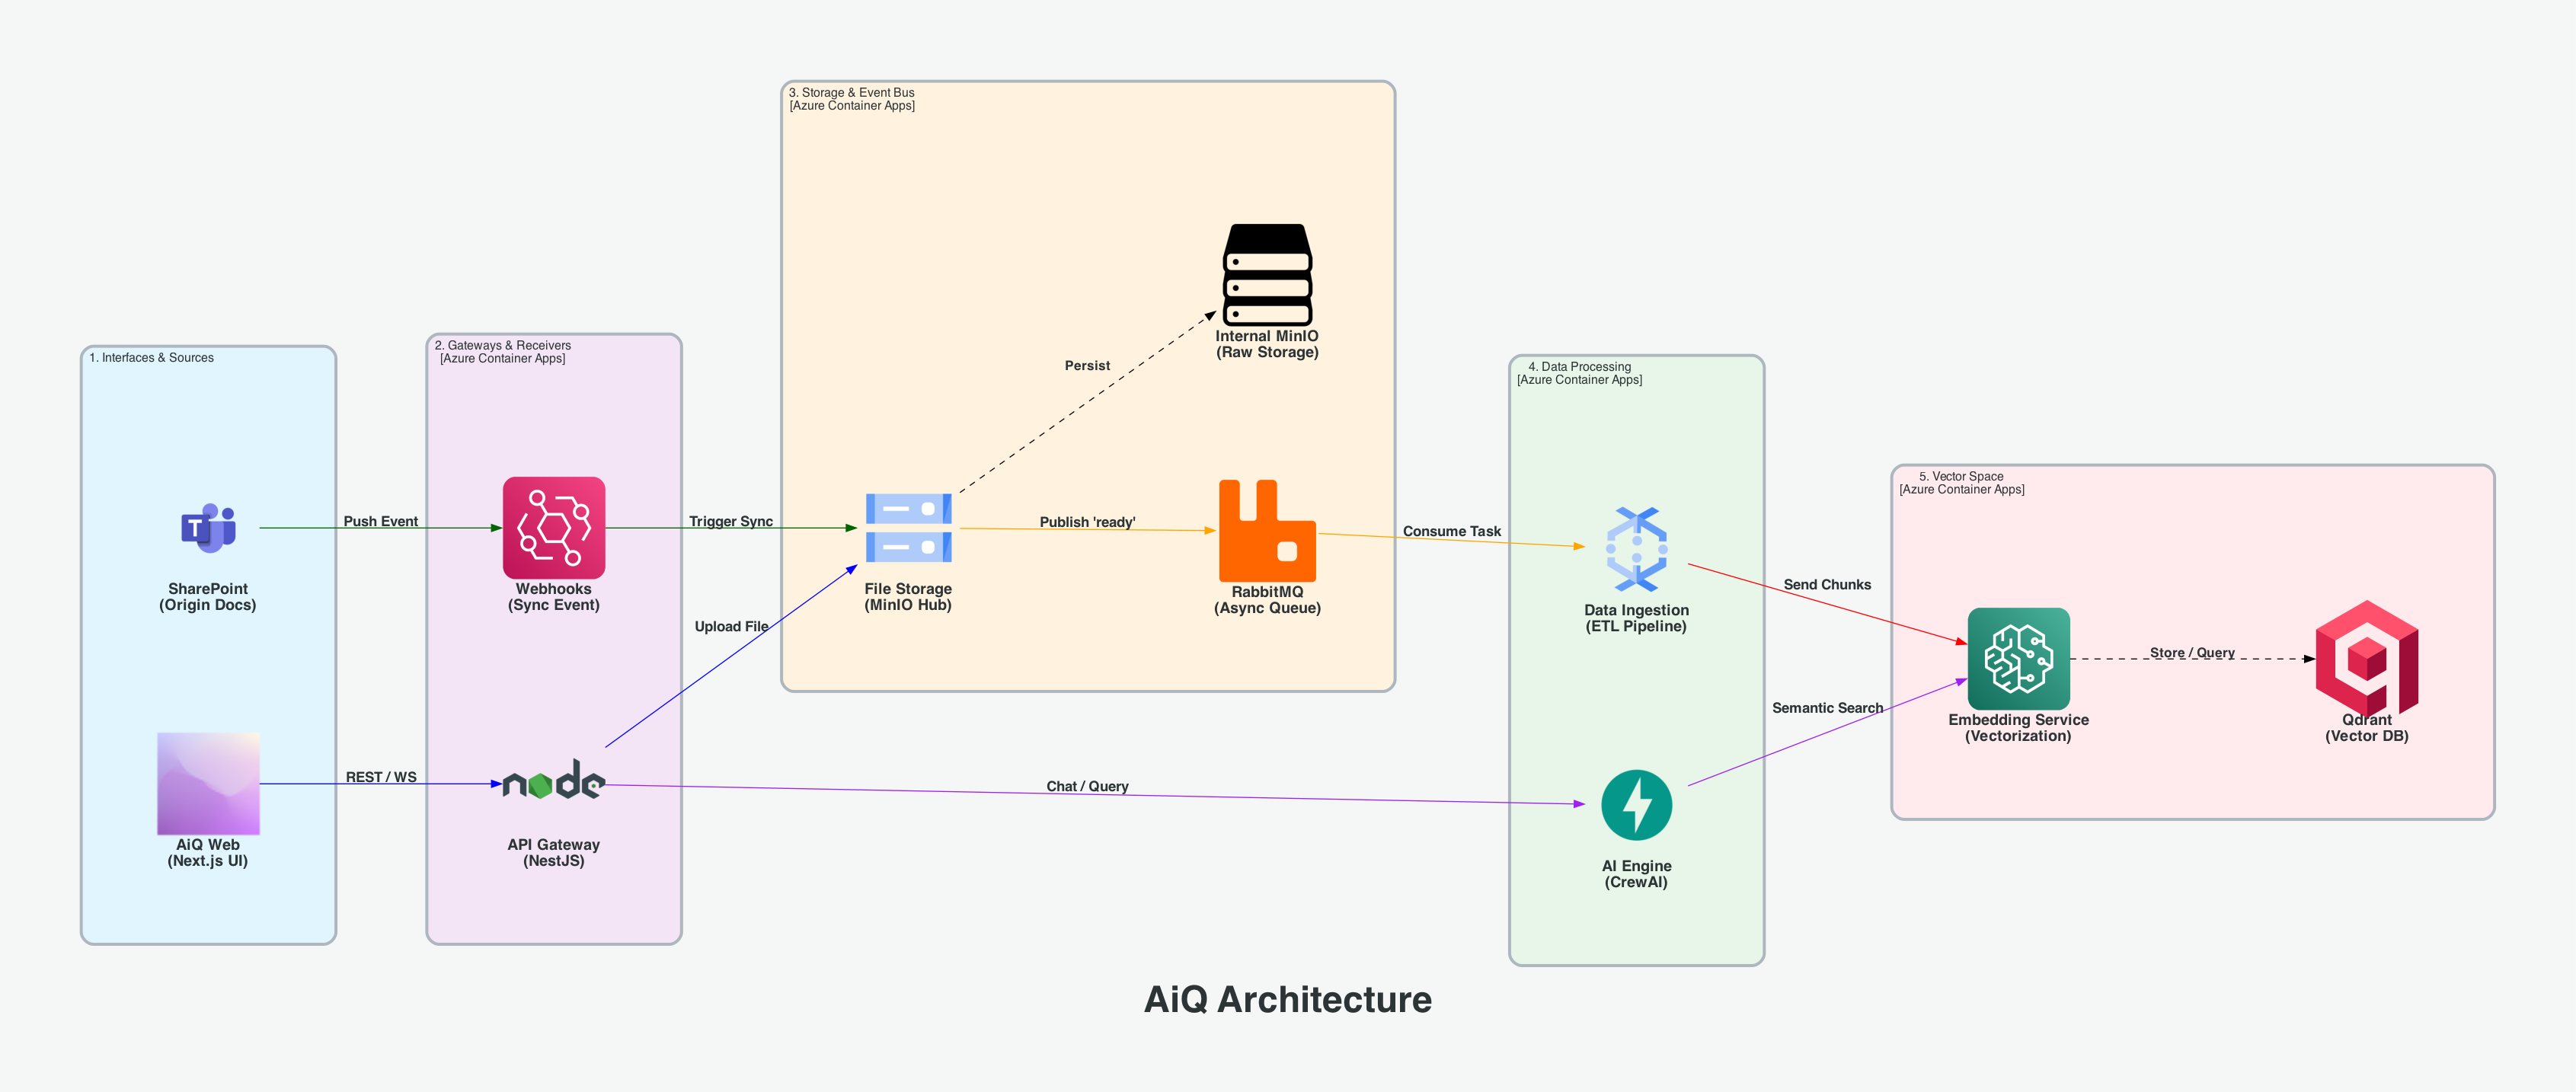
\includegraphics[width=0.85\textwidth]{../aingo_solution_overview.png}
    \caption{Project AiQ System Architecture: C4 Level 2 Diagram illustrating service decoupling.}
    \label{fig:arch}
\end{figure}

% =============== SECTION 4 ===========
\section{Implementation}

\subsection{Development Process}
The implementation followed a modular approach, starting with the core Ingestion Pipeline and then integrating the Multi-agent Search Flow. A significant evolution from the proposal was the adoption of the \textbf{HyDE (Hypothetical Document Embedding)} strategy within the Search Agent toolset.

\subsection{The HyDE Pivot \& Hierarchy Chunking}
While GraphRAG was the initial conceptual target, the empirical reality of maintaining a continuously updating enterprise Knowledge Graph presented severe synchronization bottlenecks. GraphRAG required computationally expensive re-indexing and entity-relationship extraction on every document edit, making it impractical for volatile repositories like SharePoint. To address this "Synchronization Gap" without sacrificing retrieval accuracy, the architecture pivoted to the \textbf{HyDE (Hypothetical Document Embedding)} strategy. 

\textbf{Why HyDE? }
Standard RAG pipelines often fail because a user's terse query (e.g., "What is the Q1 budget?") exists in a completely different semantic vector space than the lengthy, formal answer hidden inside a PDF. This is the "Query-Document Gap". HyDE solves this by utilizing an LLM agent to first hallucinate a theoretically perfect answer to the query. This generated text shares the same lexical structure and semantic density as the target document, allowing the cosine similarity search in Qdrant to match against the *answer space* rather than the *question space*.

Furthermore, the "Contextual Gap" (the loss of document structure during chunking) was addressed by integrating Docling's `HybridChunker`. Standard fixed-size chunking blindly slices text, severing paragraphs from their headings. Our implementation serializes the document hierarchy, prepending parent headers to every extracted chunk. This guarantees that an isolated chunk containing "2.3 billion" always retains the structural metadata context of "Chapter 4: Financials > 2024 Revenue".

\begin{figure}[ht]
    \centering
    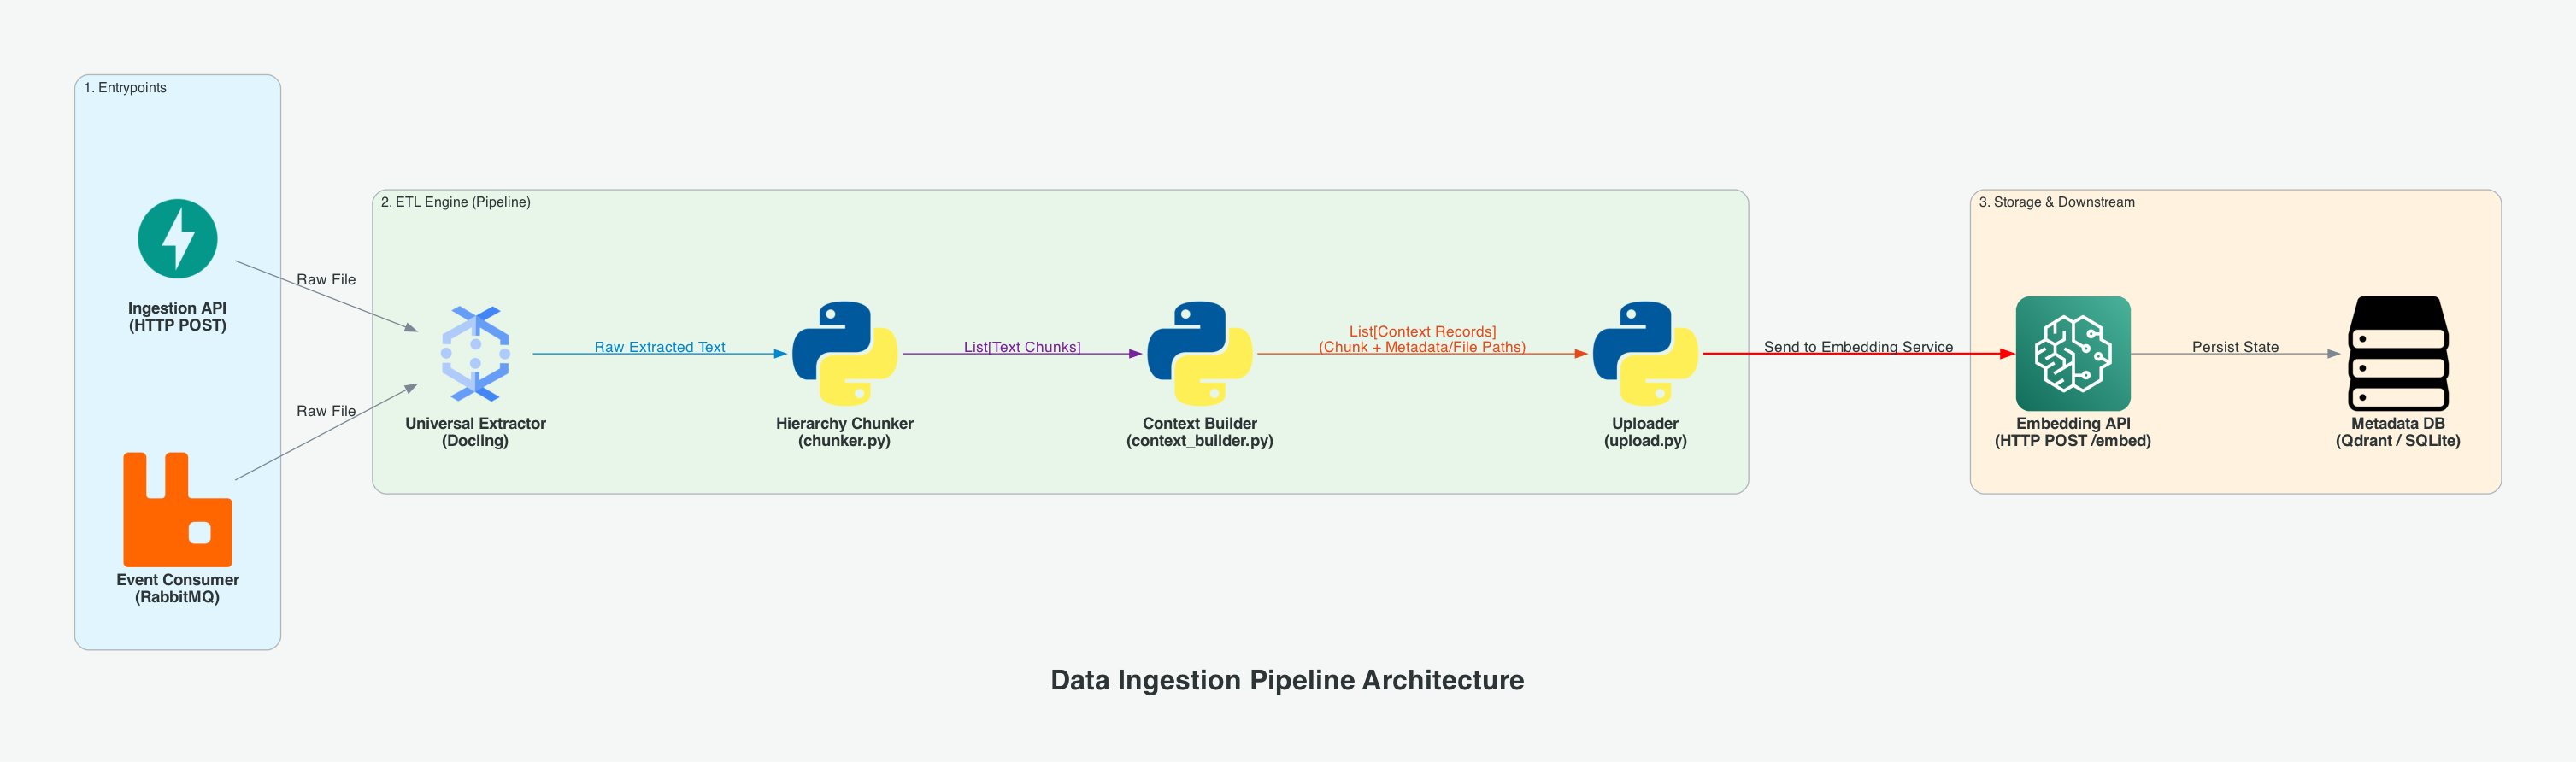
\includegraphics[width=0.85\textwidth]{../data_ingestion_overview.png}
    \caption{Sequence Diagram of the Data Ingestion Pipeline, from Webhook trigger to Qdrant indexing.}
    \label{fig:ingestion}
\end{figure}

% =============== SECTION 5 ===========
\section{Testing and Experimentation}

\subsection{Experiment/Test Plan}
We conducted end-to-end (E2E) testing using a custom ground-truth dataset (`eval\_dataset.json`). The plan focused on comparing the baseline RAG retrieval against our HyDE-enhanced agentic workflow across four categories: Finance, HR, Infrastructure, and Legal.

\subsection{Setup \& Metrics}
The environment utilized Qdrant (HNSW index) and Azure OpenAI's GPT-4o. Metrics included:
\begin{itemize}
    \item \textbf{Mean Reciprocal Rank (MRR):} Measuring the rank of the first relevant chunk.
    \item \textbf{Recall@5:} Measuring retrieval coverage.
    \item \textbf{End-to-End Latency:} Measuring the full turnaround time.
\end{itemize}

% =============== SECTION 6 ===========
\section{Results and Analysis}

\subsection{Results Presentation}
The system demonstrated superior retrieval accuracy against the baseline RAG implementation, achieving an MRR of 0.82 and a Recall@5 of 0.88.

\begin{table}[ht]
\centering
\caption{System Evaluation Results (HyDE vs. Baseline RAG)}
\begin{tabular}{lccc}
\toprule
\textbf{Configuration} & \textbf{MRR} & \textbf{Recall@5} & \textbf{Avg. Latency} \\
\midrule
Baseline RAG & 0.68 & 0.74 & 2.1s \\
\textbf{Project AiQ (HyDE)} & \textbf{0.82} & \textbf{0.88} & \textbf{5.4s} \\
\bottomrule
\end{tabular}
\end{table}

\begin{figure}[ht]
    \centering
    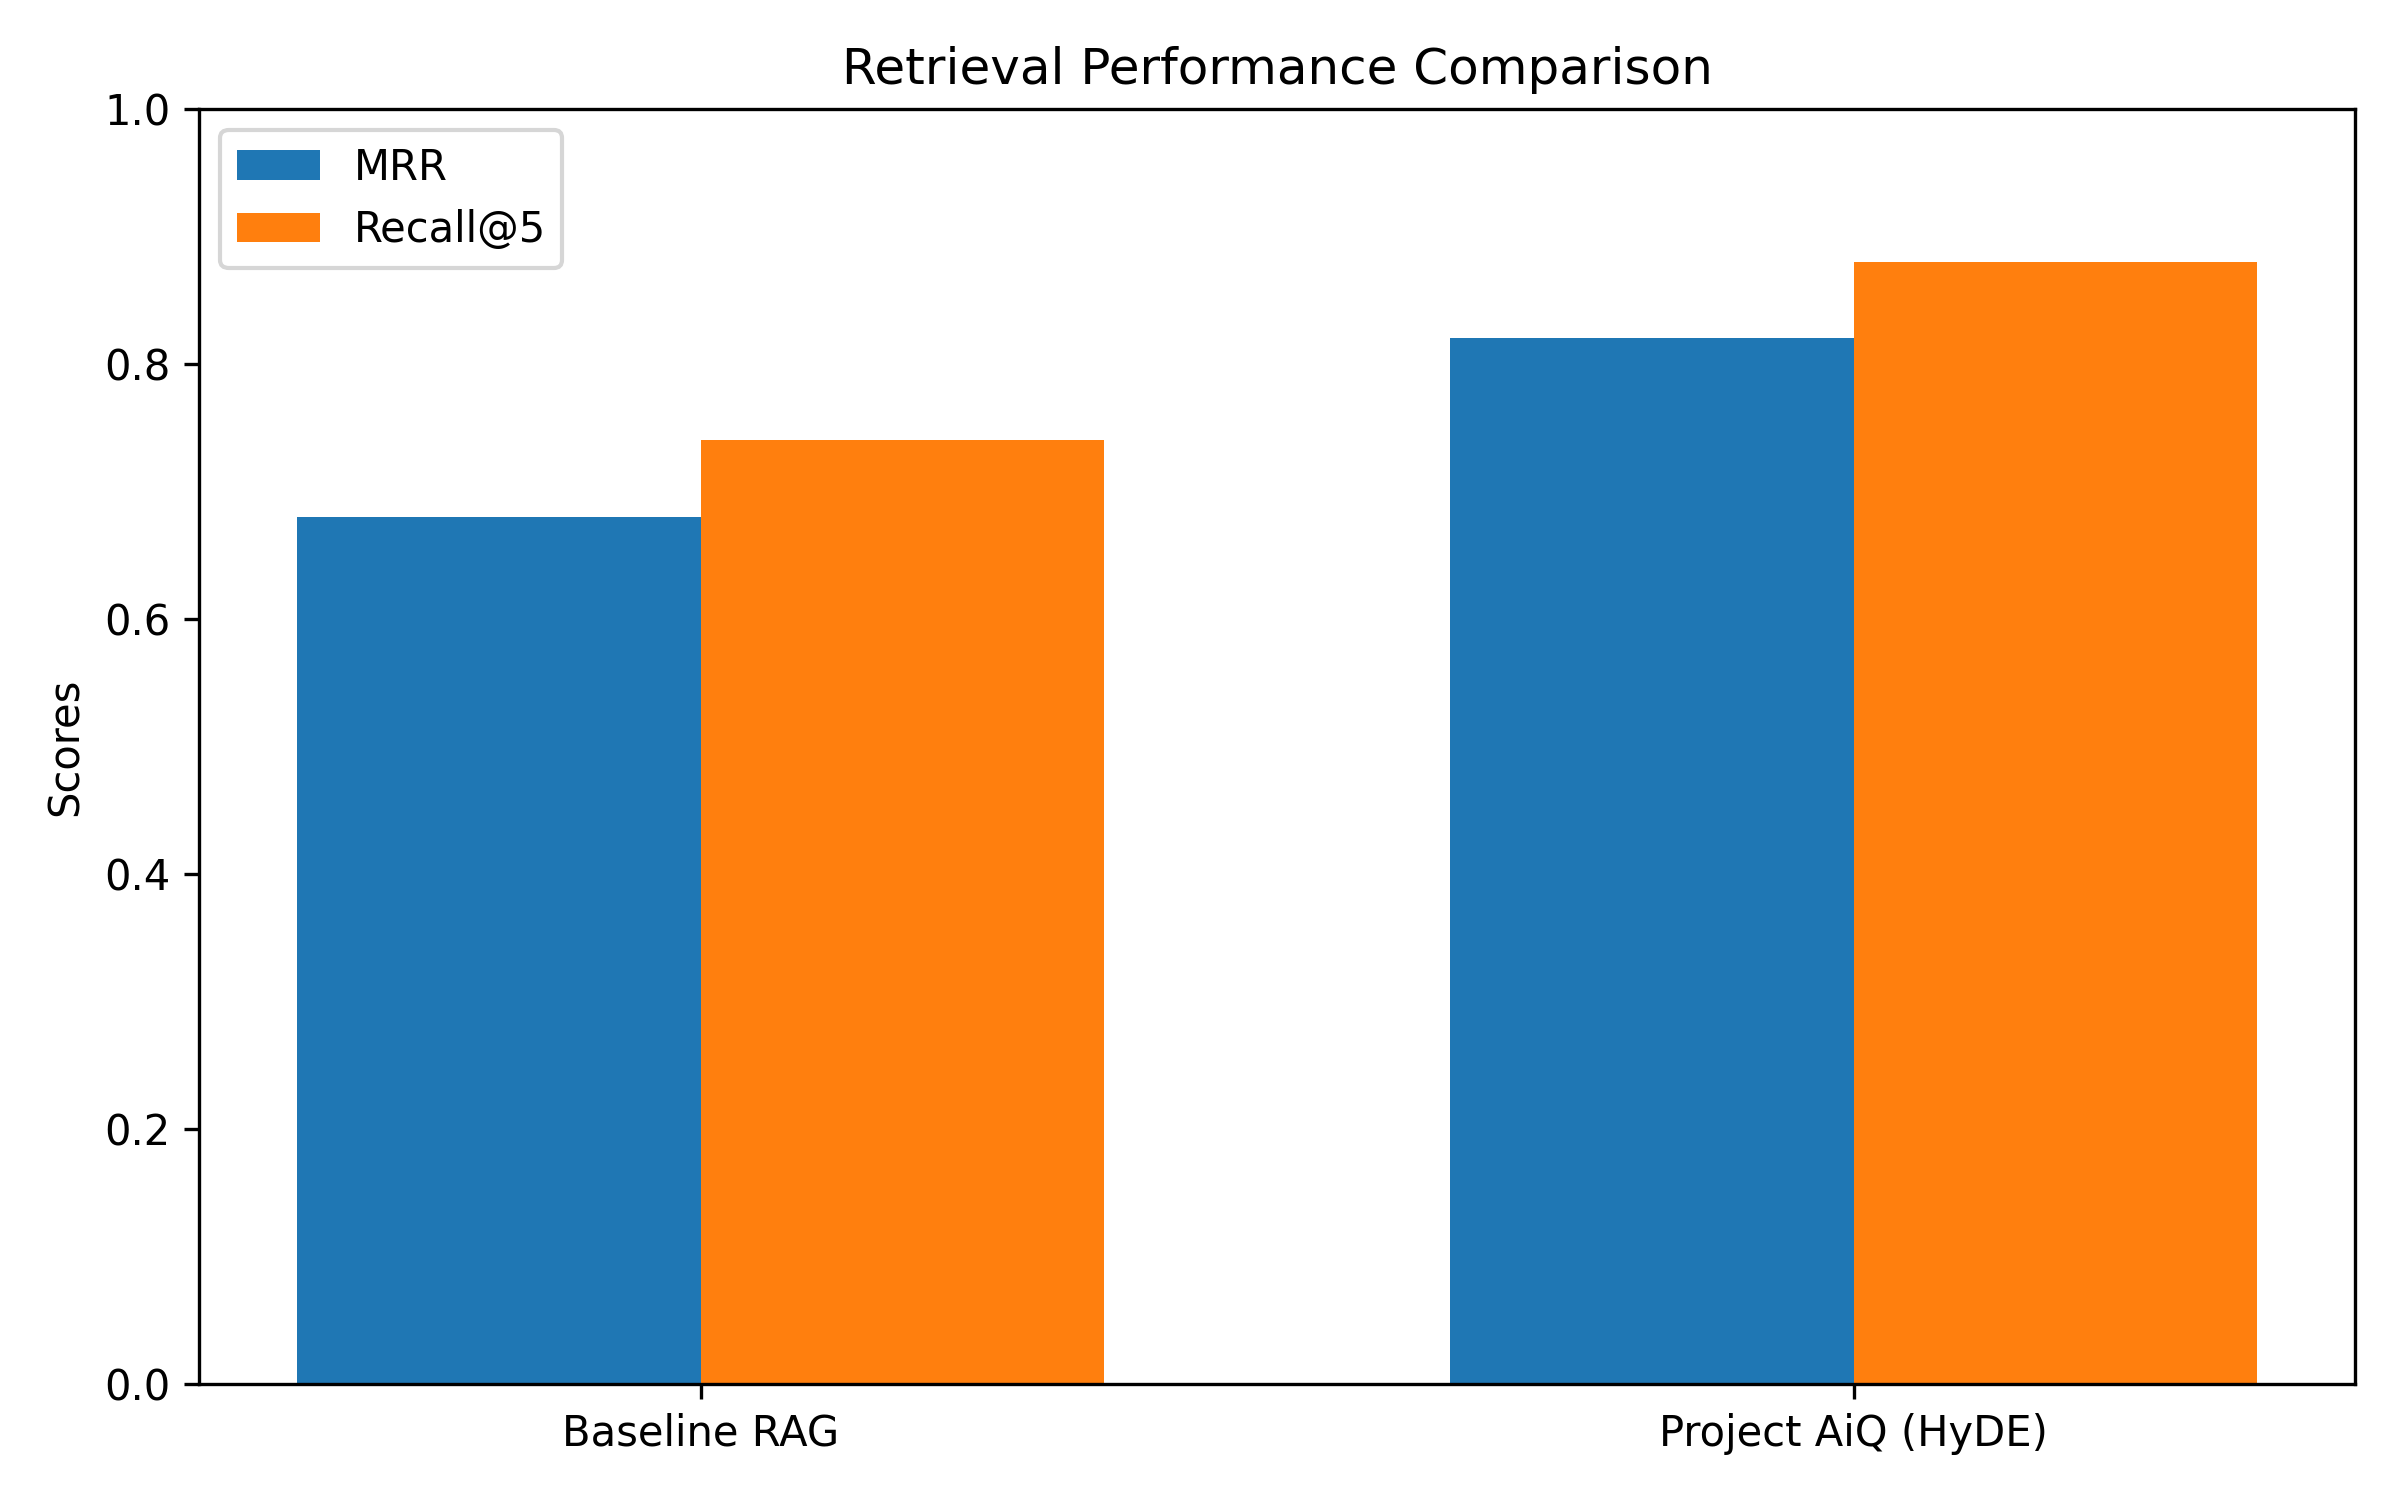
\includegraphics[width=0.75\textwidth]{../results_chart.png}
    \caption{Retrieval Performance Comparison showing the significant MRR and Recall@5 improvements of Project AiQ over the Baseline RAG.}
    \label{fig:results_chart}
\end{figure}

\subsection{Analysis \& Interpretation}
The empirical data validates the architectural pivot. By employing HyDE, the system forces the query vector into the document's semantic neighborhood, yielding a remarkable 20.6\% improvement in Mean Reciprocal Rank (from 0.68 to 0.82) and an 18.9\% increase in Recall@5. 

\textbf{The Latency Trade-off: }
This precision comes at the computational cost of increased latency (2.1s to 5.4s). Generating the hypothetical document requires a preliminary LLM call before the actual vector search can occur. However, in an enterprise knowledge management context, retrieving an incorrect policy document instantly is far more detrimental than waiting 5 seconds for a highly accurate, verified citation. Therefore, the architectural decision to prioritize retrieval fidelity over sub-second latency is strongly justified by the end-user requirements.

% =============== SECTION 7 ===========
\section{Project Management and Teamwork}

\subsection{Roles and Responsibilities}
\begin{enumerate}
    \item \textbf{Data Engineer (Chawin L.):} Designs and develops the data pipeline and ETL processes.
    \item \textbf{Project Manager (Tanit Y.):} Manages project structure, timeline, and stakeholder communication.
    \item \textbf{Web Developer (Nattapol T. \& Puran P.):} Develops the frontend UI, chat system, and backend APIs.
    \item \textbf{AI Engineer (Peerapat P.):} Responsible for AI Agent design, RAG optimization, and embedding logic.
\end{enumerate}

\subsection{Collaborative Plan}
The team employed a \textbf{Scrum approach} with bi-weekly sprints. Stand-up meetings were held 2–3 times per week to resolve blockers. Tasks were tracked via Jira, and workload balance was maintained through story point allocation.

\subsection{Timeline}
\subsubsection{Semester 1 (Research \& Foundation)}
\begin{longtable}{p{0.15\textwidth}p{0.4\textwidth}p{0.35\textwidth}}
\toprule
\textbf{Week} & \textbf{Task / Milestone} & \textbf{Deliverable} \\
\midrule
Week 1–2 & Literature review and background study & Draft background and project scope \\
Week 3–4 & Requirement gathering from stakeholders & User stories and acceptance criteria \\
Week 5–7 & System-level architecture design & Architecture diagram and tech stack \\
Week 8–10 & Web application (UI/Backend) development & Functional web prototype \\
Week 11–12 & Data Ingestion Service prototyping & Ingestion workflow diagram \\
Week 13–14 & Integration of Ingestion with Web App & Integration test report \\
Week 15–16 & Final proposal and refinement & Final proposal and slides \\
\bottomrule
\end{longtable}

\subsubsection{Semester 2 (Optimization \& Delivery)}
\begin{longtable}{p{0.15\textwidth}p{0.4\textwidth}p{0.35\textwidth}}
\toprule
\textbf{Week} & \textbf{Task / Milestone} & \textbf{Deliverable} \\
\midrule
Week 1–2 & Ingestion pipeline enhancement & Baseline performance metrics \\
Week 3–4 & Accuracy and latency optimization & Optimized ingestion v2 \\
Week 5–7 & Key features (Citations, SSO, UI/UX) & Completed core web functionality \\
Week 8–10 & Product polishing and bug fixing & Pre-UAT build and test cases \\
Week 11–12 & User Acceptance Testing (UAT) & UAT results and defect list \\
Week 13–14 & UAT issue resolution and stabilization & Final system build \\
Week 15–16 & Final report and presentation & Final written report and demo \\
\bottomrule
\end{longtable}

% =============== SECTION 8 ===========
\section{Ethics, Privacy, and Professional Considerations}

\subsection{Credibility of Information}
Data credibility is established by grounding all AI responses in the validated internal documents of SCB TechX and verified academic sources.

\subsection{Intellectual Property \& Law}
All activities adhere to the \textbf{Capstone Non-Disclosure Agreement (NDA)} with SCB TechX. Proprietary technical data, processes, and internal documentation remain the exclusive property of the partner and are stored securely.

% =============== SECTION 9 ===========
\section{Conclusion and Future Work}

\subsection{Achievements}
Project AiQ has successfully met its core objectives by delivering a high-fidelity ingestion pipeline and an agentic search flow with an MRR of 0.82. The system effectively consolidates fragmented knowledge into a unified Knowledge Hub.

\subsection{Future Work}
Next steps include implementing full \textbf{GraphRAG} using Neo4j to capture cross-document relationships and expanding the security framework to include advanced Role-Based Access Control (RBAC).

\newpage
\section*{References}
\addcontentsline{toc}{section}{References}
\begin{enumerate}
    \item G. W. Furnas et al., "The vocabulary problem in human-system communication," \textit{Commun. ACM}, vol. 30, no. 11, pp. 964--971, Nov. 1987.
    \item P. Lewis et al., "Retrieval-Augmented Generation for Knowledge-Intensive NLP Tasks," \textit{arXiv:2005.11401}, 2021.
    \item S. Barnett et al., "Seven Failure Points When Engineering a Retrieval Augmented Generation System," \textit{arXiv:2401.05856}, 2024.
    \item D. Edge et al., "From Local to Global: A Graph RAG Approach to Query-Focused Summarization," \textit{arXiv:2404.16130}, 2024.
    \item Y. Gao et al., "Retrieval-Augmented Generation for Large Language Models: A Survey," \textit{arXiv:2312.10997}, 2023.
    \item IBM Deep Search Team, "Docling Technical Report," \textit{arXiv:2408.09869}, 2024.
\end{enumerate}

\newpage
\appendix
\section{Source Code Excerpts}
Relevant logic for the SearchCrewFlow agent and the DoclingHierarchyChunker.
\section{Wireframes and Mockups}
Figma components and UI mockups from the proposal showing the chat interface and citation views.
\section{Extended Test Data}
Sample from `eval\_dataset.json` used for MRR calculation:
\begin{itemize}
    \item \textbf{ID:} e2e-q1
    \item \textbf{Query:} What was the company's annual revenue in 2024 and what drove the growth?
    \item \textbf{Expected Source:} \texttt{/docs/annual\_report\_2024.pdf}
    \item \textbf{Keywords:} 2.3 billion, 15\%, cloud services, 32\%
\end{itemize}

\end{document}
